%\title{LaTeX Portrait Poster Template}
%%%%%%%%%%%%%%%%%%%%%%%%%%%%%%%%%%%%%%%%%
% a0poster Portrait Poster
% LaTeX Template
% Version 1.0 (22/06/13)
%
% The a0poster class was created by:
% Gerlinde Kettl and Matthias Weiser (tex@kettl.de)
% 
% This template has been downloaded from:
% http://www.LaTeXTemplates.com
%
% License:
% CC BY-NC-SA 3.0 (http://creativecommons.org/licenses/by-nc-sa/3.0/)
%
%%%%%%%%%%%%%%%%%%%%%%%%%%%%%%%%%%%%%%%%%

%----------------------------------------------------------------------------------------
%	PACKAGES AND OTHER DOCUMENT CONFIGURATIONS
%----------------------------------------------------------------------------------------

\documentclass[a0,portrait]{a0poster}

\usepackage{multicol} % This is so we can have multiple columns of text side-by-side
\columnsep=100pt % This is the amount of white space between the columns in the poster
\columnseprule=3pt % This is the thickness of the black line between the columns in the poster

\usepackage[svgnames]{xcolor} % Specify colors by their 'svgnames', for a full list of all colors available see here: http://www.latextemplates.com/svgnames-colors

\usepackage{times} % Use the times font
%\usepackage{palatino} % Uncomment to use the Palatino font
\usepackage[spanish]{babel}
\usepackage[utf8]{inputenc}
\usepackage{amsmath}
\usepackage{graphicx} % Required for including images
\graphicspath{{figures/}} % Location of the graphics files
\usepackage{booktabs} % Top and bottom rules for table
\usepackage[font=small,labelfont=bf]{caption} % Required for specifying captions to tables and figures
\usepackage{amsfonts, amsmath, amsthm, amssymb} % For math fonts, symbols and environments
\usepackage{wrapfig} % Allows wrapping text around tables and figures

\begin{document}

%----------------------------------------------------------------------------------------
%	POSTER HEADER 
%----------------------------------------------------------------------------------------

% The header is divided into two boxes:
% The first is 75% wide and houses the title, subtitle, names, university/organization and contact information
% The second is 25% wide and houses a logo for your university/organization or a photo of you
% The widths of these boxes can be easily edited to accommodate your content as you see fit

\begin{minipage}[b]{0.75\linewidth}
\VeryHuge \color{NavyBlue} \textbf{Factorizaciones matriciales
aproximadas aplicadas en el reconocimiento de g\'enero} \color{Black}\\ % Title
\Huge\textit{Factorizaci\'on no negativa de Matrices y una versi\'on local}\\[2.4cm] % Subtitle
\huge \textbf{Jorge Luis Ramos Zavaleta}\\[0.5cm] % Author(s)
\huge Centro de Investigaci\'on en Matem\'aticas (CIMAT A.C.), Unidad Monterrey\\[0.4cm] % University/organization
\Large \texttt{jorge.ramos@cimat.mx} \\
\end{minipage}
%
\begin{minipage}[b]{0.25\linewidth}

\includegraphics[width=9cm]{logo_cimat.jpg}\ 

\includegraphics[width=9cm]{logo_U_Mty.png}\\
\end{minipage}

\vspace{1cm} % A bit of extra whitespace between the header and poster content

%----------------------------------------------------------------------------------------

\begin{multicols}{3} % This is how many columns your poster will be broken into, a portrait poster is generally split into 2 columns

%----------------------------------------------------------------------------------------
%	ABSTRACT
%----------------------------------------------------------------------------------------

\color{Navy} % Navy color for the abstract

\begin{abstract}
Un rostro puede ser representado conceptualmente como una conjunto de partes distribuídas de manera esparcida: ojos, nariz, boca, etc. Los humanos tenemos la habilidad de encontrar patrones en las caras lo que nos permite diferenciar entre el rostro de un hombre y el de una mujer. El siguiente reporte presenta los resultados de aplicar NMF(non-negative matrix factorization), LNMF(Local NMF) y PCA a diversas imágenes de rostros de hombres y mujeres con el fin de generar un clasificador de género comparando los 3 métodos para conocer su efectividad en dicha tarea.
\end{abstract}
%----------------------------------------------------------------------------------------
%	INTRODUCTION
%----------------------------------------------------------------------------------------
\color{Black} % SaddleBrown color for the introduction
\section*{Introducci\'on}
Debido a los problemas que se generan en altas dimensiones ya sea por redundancias o superposiciones de características, el análisis de objetos en el espacio de los datos originales puede ser computacionalmente exhaustivo. Por lo que problemas que requieren el análisis de imágenes en particular de rostros generalmente el problema es convertido a uno con un subespacio de dimensión más baja para que sea más facilmente tratable.\newline

Asimismo una representación en un subespacio suficiente bueno puede exponer estructuras escondidas y características inherentes al tipo de objetos con el que se quiere trabajar. Inclusive puede considerarse alguna bondad de dicho subespacio en el que trabajar con diferentes variaciones como de iluminación o traslaciones sea mucho mas sencillo que si se tratara con el espacio original.\newline

Esto nos lleva a establecer que la elección de una apropiada representación de los datos en un subespacio de menor dimensión que el original puede volverse imperativo para el éxito y eficacia de un sistema de reconocimiento de objetos o rostros como es nuestro caso.
%----------------------------------------------------------------------------------------
%	GEOLOGY
%----------------------------------------------------------------------------------------
\color{Black} % DarkSlateGray color for the rest of the content

\section*{PCA, NMF y LNMF}
PCA es uno de los métodos más usados en estadística y es por ello que es muy conocido y aplicado para hacer reducción de dimensión así como para intentar encontrar características en datos multivariados. El método consiste en encontrar direcciones sobre las cuales las proyecciones de los datos generen la máxima varianza.\newline

El enfoque de detección de rostros usando PCA es muy conocido y recibe el nombre de eigenfaces. Es un esquema muy simple el que se usa para aplicar PCA a diversos rostros. Para ello se genera una matriz con cada rostro vectorizado y colocado como una columna de dicha matriz después se calcula la imagen media y se le resta a cada imagen de la matriz para centrar las imágenes y evitar problemas dados por traslaciones. A esta matriz centrada se le calcula su factorización SVD y se considera el número de componentes a usar dependiendo el criterio que se elija para esto.\newline

Al igual que PCA tanto NMF como su versión local son esquemas de aproximación de una matriz considerando un rango más bajo que el de la matriz original. Aun cuando se sabe que PCA (SVD) tiene la mejor aproximaci\'on de rango bajo de una matriz la naturaleza inherente de no negatividad de algunas estructuras de datos permite entrever la utilidad de estos esquemas multivariados que consideran dicha propiedad.\newline
\begin{center}\vspace{0.5cm}
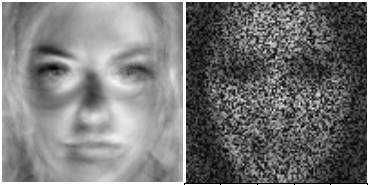
\includegraphics[width=0.7\linewidth]{Sin_nombre}
\captionof{figure}{\color{NavyBlue} Izquierda: Eigenface obtenida utilizando PCA. Derecha: Atributos obtenidos usando NMF.}
\end{center}%\vspace{1cm}


%----------------------------------------------------------------------------------------
%	GEOTHERMAL DATA
%----------------------------------------------------------------------------------------
\subsection*{NonNegative Matrix Factorization (NMF)}
A finales de los 1970's ya se había planteado la idea de usar una factorización de matrices con restricción de no negatividad, sin embargo el problema de optimización que esto conlleva es de tipo Np-hard por lo que se abandono la idea, y fue hasta que en 1999 se publica un resultado donde se propone una forma de resolver dicho problema de optimización haciendo uso de una regla de actualización multiplicativa. \newline

A partir de dicho resultado se ha comenzado una extensa investigación este tipo de aproximación de rango bajo y de como generar extensiones del método para considerar problemas más complejos.\newline

El problema que se intenta resolver es
$$min \ D(X|BH), \ \ \ \ \ s. \ a. \ B\geq 0 \ y \ H\geq 0$$
Con $$D(X|BH)=\sum_{i,j}\left(X_{ij}log\frac{X_{ij}}{BH_{ij}} - X_{ij} + BH_{ij} \right)$$
Y para ello se hace uso de una actualización multiplicativa 
$$h_{pj}=h_{pj}\sum_{i=1}^n \left(\frac{b_{ip}a_{ij}}{\sum_{k=1}^r b_{ik}h_{kj}}\right), \ \ b_{ip}=b_{ip}\sum_{j=1}^m \left(\frac{a_{ij}h_{pj}}{\sum_{k=1}^r b_{ik}h_{kj}} \right)$$ $$b_{ip}=\frac{b_{ip}}{\sum_{k=1}^n b_{kp}}$$

Haciendo uso de estas funciones de actualización multiplicativa se tiene garantizado que la divergencia de Kullback-Leibler sea no creciente con cada actualización.\newline

A partir del trabajo de Lee se han encontrado otras formas de resolver el problema de optimización. Sin embargo, uno de los problemas asociados a estos nuevos descubrimientos es que la factorización no es única.

%------------------------------------------------

\subsection*{Local NMF}
Local NMF es una extensión del algoritmo original de NMF en el que se busca que se haga una búsqueda en el espacio local para encontrar características locales en lugar de las características globales que encuentran PCA y NMF. En nuestro problema a resolver, permitiría encontrar características específicas que pueden determinar lo que define un rostro masculino o un rostro femenino.\newline

Dado que se trata de una extensión de NMF entonces se tienen condiciones de optimalidad mayores que los de NMF. Dado que $$A\approx BH$$ Definimos: $$U=B^T B \ y \ V=HH^t$$ Entonces para lograr que se establezca una búsqueda local se requiere que se cumplan las siguientes restricciones
\begin{itemize}
\item Máxima esparcidad en H.- Esta se logra minimizando la diagonal de U
\item Máxima expresividad en B.-Esta se logra maximizando la traza de V
\item Ortogonalidad de las bases.- Esta se logra minimizando la suma de las entradas de la matriz U
\end{itemize}
por lo que la divergencia de Kullback-Leibler toma la siguiente forma
\begin{multline*}D(X|BH)=\sum_{i,j}\left(X_{ij}log\frac{X_{ij}}{BH_{ij}} - X_{ij} + BH_{ij} \right) \\ +\alpha\sum_{i,j} u_{ij}-\beta\sum_{i}v_{ii}\end{multline*} Por lo que el problema de minimización a resolver es similar al que se resuelve con NMF y tambien puede resolverse usando una regla multiplicativa.

\section*{Comparaci\'on de los m\'etodos en la detecci\'on de g\'enero}
Un problema básico que se encuentra al querer hacer comparaciones entre métodos, como es nuestro caso, es que se deben considerar igualdad de condiciones para que los métodos no se vean comprometidos por alguna consideración que les pueda afectar directamente en su funcionamiento y en este caso en su nivel de precisión al clasificar.\newline

Para esto se eligi\'o realizar la detección del rostro en la imagen haciendo uso de del método de Cascada de Haar.\newline

\begin{center}\vspace{0.5cm}
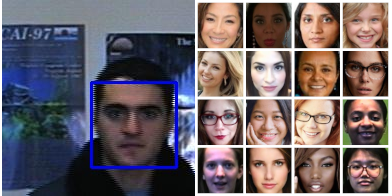
\includegraphics[width=0.7\linewidth]{collage3}
\captionof{figure}{\color{NavyBlue} Izquierda: Rostro detectado haciendo uso de la cascada de Haar. Derecha: Muestra de rostros de mujeres obtenidos usando la Cascada de Haar.}
\end{center}%\vspace{1cm}


%----------------------------------------------------------------------------------------
%	CONCLUSIONS
%----------------------------------------------------------------------------------------

\color{SaddleBrown} % SaddleBrown color for the conclusions to make them stand out

\section*{Resultados}
Para la implementación se consideraron 306 imágenes de hombres y mujeres en total. Para establecer la clasificación por género se genero un pequeño ensamble generando una base para las mujeres y otra para los hombres. A cada imagen nueva se le calcula la correlación contra cada elemento de la base de mujeres y se calcula la máxima correlación en esta base, de manera analóga se hace para la base de hombres, y el criterio de decisión es como sigue
\begin{multline*}
Max(Corr(x,Mujeres))>Max(Corr(x,hombres))\rightarrow M\\ Max(Corr(x,Mujeres))<Max(Corr(x,hombres))\rightarrow H
\end{multline*}
En caso de empate se elige aleatoriamente de manera uniforme.
\color{Black} % Set the color back to DarkSlateGray for the rest of the content
\begin{center}\vspace{0.5cm}
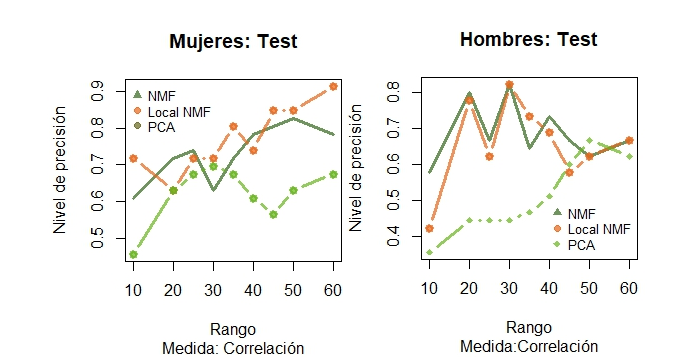
\includegraphics[width=1.0\linewidth]{resultados}
\captionof{figure}{\color{NavyBlue} Izquierda: Nivel de precisi\'on obtenido para el conjunto de rostros de mujer en el conjunto de prueba para diferentes rangos. Derecha: Nivel de precisi\'on obtenido para el conjunto de prueba para hombres con distintos rangos.}
\end{center}%\vspace{1cm}
\begin{center}\vspace{0.5cm}
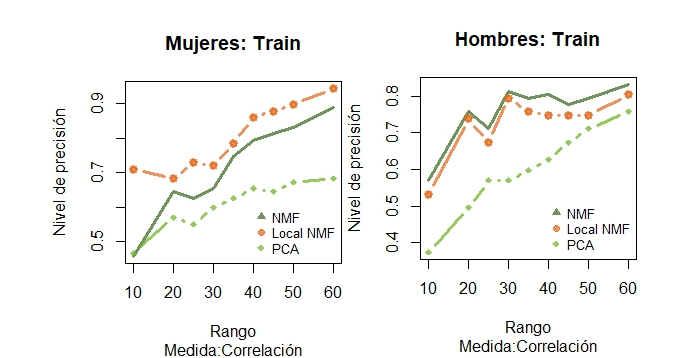
\includegraphics[width=1.0\linewidth]{resultados2}
\captionof{figure}{\color{NavyBlue} Izquierda: Nivel de precisi\'on obtenido para el conjunto de rostros de mujer en el conjunto de entrenamiento para diferentes rangos. Derecha: Nivel de precisi\'on obtenido para el conjunto de entrenamiento para hombres con distintos rangos.}
\end{center}%\vspace{1cm}

\color{SaddleBrown} 
Puede observarse que en el caso de mujeres LNMF logro encontrar atributos muy espec\'ficos en sus rostros por lo que en general supera a PCA y a NMF. Mientras que en el caso de los hombres parece no haber caracter\'isticas tan distintivas en sus rostros por lo que clasifica al mismo nivel que NMF. Pero ambos casos logran superar en general a PCA mostrando la utilidad de este enfoque de no negatividad.
%----------------------------------------------------------------------------------------
%	FORTHCOMING RESEARCH
%----------------------------------------------------------------------------------------

 %----------------------------------------------------------------------------------------
%	REFERENCES
%----------------------------------------------------------------------------------------
\color{Black} 
\section*{Referencias}
\begin{itemize}
\item Ding, C. H., Li, T., \& Jordan, M. I. (2010). Convex and semi-nonnegative matrix factorizations. IEEE transactions on pattern analysis and machine intelligence, 32(1), 45-55.
\item Feng, T., Li, S. Z., Shum, H. Y., \& Zhang, H. (2002). Local non-negative matrix factorization as a visual representation. In Development and Learning, 2002. Proceedings. The 2nd International Conference on (pp. 178-183). IEEE.
\item Lee, D. D., \& Seung, H. S. (1999). Learning the parts of objects by non-negative matrix factorization. Nature, 401(6755), 788. 
\item Li, S. Z., Hou, X. W., Zhang, H. J., \& Cheng, Q. S. (2001). Learning spatially localized, parts-based representation. In Computer Vision and Pattern Recognition, 2001. CVPR 2001. Proceedings of the 2001 IEEE Computer Society Conference on (Vol. 1, pp. I-I). IEEE.

\end{itemize}
%\nocite{*} % Print all references regardless of whether they were cited in the poster or not
%\bibliographystyle{plain} % Plain referencing style
%\bibliography{sample} % Use the example bibliography file sample.bib

%----------------------------------------------------------------------------------------

\end{multicols}
\end{document}